\section{Applications on Uchuu-ZTF Mocks}

\subsection{Uchuu-ZTF Mocks} \label{sec:uchuu_ztf}

The ZTF simulations are designed to test the impact of ZTF-supernovae peculiar velocities in a cosmological analysis are called DC PV (Data Challenge 
Peculiar Velocity). These are generated within the ZTF collaboration mainly to test the methods to infer $f\sigma_8$. 
The DC PV simulations are done similarly to the DC simulations  
described in Chapter 4 with the main differences being that supernovae are simulated on top of large scale structures instead of a uniform distribution. 
For that, we use the Uchuu N-body simulation 
(\cite{Ishiyama_2021}), a high fidelity N-body dark matter simulation\footnote{N-body and hydrodynamical simulations 
are considered the highest fidelity simulations we can get to describe structure formation as they solving the equations of motion for each particle/fluid without any 
approximations or grid mesh} 
in a $(2 \text{Gpc}.h^{-1})^3$ box with 2.1 trillion particles that can be seen in Figure \ref{fig:uchuu_nbody} . 
The full box is then subdivided into 27 subboxes where the supernovae are simulated up to a redshift of $z=0.11$, giving 27 quasi-independent 
realizations of the DC PV. 
Each supernova is simulated at the location of a dark matter halo is and is assigned the halo's velocity. This allows us to add proper motion to supernovae 
that is driven by structure formation.\\

\begin{figure}[ht]
    \centering
    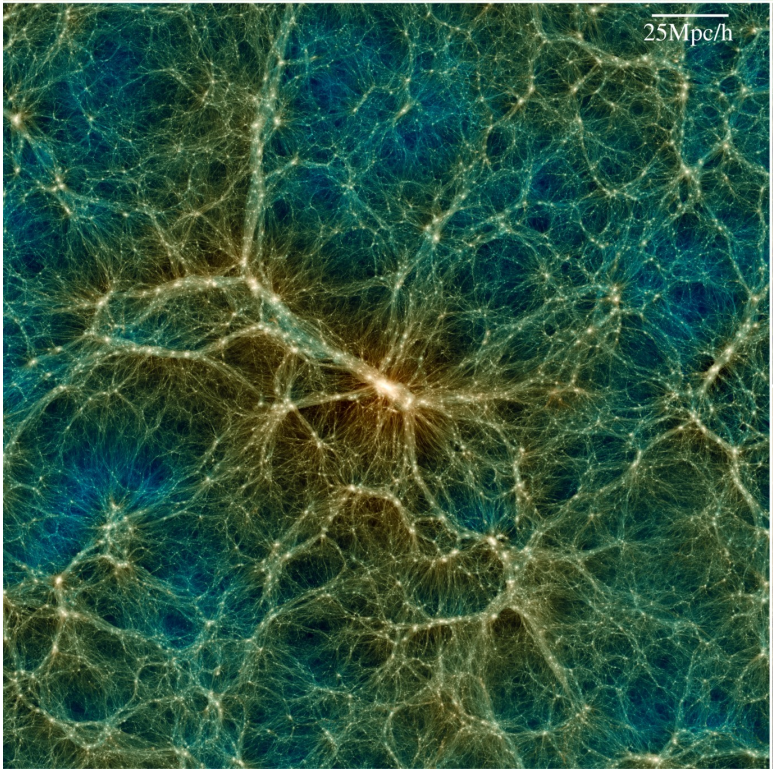
\includegraphics[width=0.7\textwidth]{MainLayout/BORG_chapter/figures/uchuu_nbody.png}
    \caption{Slice taken from the Uchuu simulation covering a box of 250 $\text{Mpc}.h^{-1}$ where each point represents a particle. Taken from \cite{Ishiyama_2021}}
    \label{fig:uchuu_nbody}
\end{figure}


We opt to simplify a few aspects of the simulations in order to have an initial assessment of how well can a BORG analysis run on ZTF-like supernova. 
Firstly, we have chosen to use only the distance moduli and redshifts of supernovae as inputs in BORG, as if we were doing the analysis after having run the full 
LEMAITRE pipeline. 
One could also infer the Tripp relation parameters ($\alpha_{\text{Tripp}}$, $\beta_{\text{Tripp}}$) in BORG. 
Performing this inference at the BORG level would offer an 
additional advantage: the 3-dimensional reconstruction of the matter 
distribution in the nearby Universe provides a 
correction for inhomogeneous Malmquist bias. In standard analyses, 
Malmquist bias corrections rely on an assumed homogeneous distribution 
of matter, which can introduce systematic errors in underdense and 
overdense regions. Within BORG, the reconstructed density field 
directly encodes the inhomogeneous matter distribution along each line 
of sight, allowing a more accurate correction for the preferential 
detection of supernovae in overdense environments near the survey 
boundary.
Secondly, we do not impose the ZTF DR2 cosmology quality cuts on photometry nor the ZTF footprint, so all of the supernovae that are 
generated can be used. 
For a more realistic set of simulations, we would have to account for the geometry of the survey as well as the Milky-Way dust. This is trivial to account for, but 
for simplicity we opted not to include it. 
It consists in introducing an 
angular mask $M(\text{RA}, \text{Dec})$ in the likelihood's selection function. 
This method was applied in BORG analyses such as 
\cite{Mcalpine_2025} (Manticore-Local) and \cite{Mcalpine_2026} (Manticore-Deep). 
Finally, we simulate ZTF-like supernova up to a redshift of $z=0.11$ and draw a set of 1000 randomly selected supernovae whose observed redshift goes up to $z=0.06$ in order to 
match the expected number of supernovae in the volume-limited sample from ZTF. \\

\subsection{Forward Model Analysis: Likelihood Profile Test}

The methodology used to generate supernova in the self consistent simulations and DC PV are different as we have mentioned earlier. We want to ensure that we can 
quantify any systematic biases introduced by those differences. To do this, we start by generating an initial density field using BORG $\delta^{\text{BORG}}_{IC}$ using a 
Planck18 cosmology (\cite{Planck_2018_params}) and known bulk flow $\mathbf{V}$. The configuration of the generated field is given in Table \ref{tab:borg_nbody}. 
We then let that field evolve using LPT gravity model to obtain the evolved density field 
$\delta^{\text{BORG}}_{F}$ and velocity field $\mathbf{v}^{\text{BORG}}_{IC}$. The ZTF simulations are designed to generate the supernovae on top of an N-body simulation, so 
from the evolved density field we create a "synthetic" N-body simulation. The simplest way to do so is to take each voxel-$i$ and generate within it $N_i$ particles proportional 
to $(1+\lceil \delta^{\text{BORG}}_{F}\rceil )_i$ where $i$ denotes the voxel index. We take the ceiling of the evolved density field to ensure we get an integer number of 
particles and to have at least 1 particle in empty voxels. We also generate fewer particles than in the Uchuu simulation, around 2 million, due to memory and storage limiations. \\

\begin{table}[ht]
    \centering
    \caption{Set of parameters used to generate the "synthetic" N-body BORG simulation.}
    \label{tab:borg_nbody}
    \begin{tabular}{|l|c|}
        \hline
        Parameters & Values \\
        \hline
        Box size & $700^3 \, (\text{Mpc}.h^{-1})^3$ \\
        Generated supernovae & $\sim 1000$ \\
        Maximum supernova redshift & $z=0.06$ \\
        Gravity model & COLA \\
        Resolution & 10.9 $\text{Mpc}.h^{-1}$ \\
        $V_x$ & 0 km/s \\
        $V_y$ & 0 km/s \\
        $V_z$ & 0 km/s \\
        $\Omega_m$ & 0.31 \\
        $\sigma_8$ & 0.81 \\
        \hline
    \end{tabular}
\end{table}
We then use this "synthetic" N-body simulation to generate ZTF-like supernovae using skysurvey (\cite{Rigault_2026}) and then evaluate the BORG-supernova likelihood (Equation \ref{eqn:borg_pv_L}) 
while varying the cosmological and model parameters in BORG. We create a likelihood profile for each parameter, not only to 
determine whether the ZTF-like supernova simulations introduce systematic biases in BORG but also to help us understand how we can relate some of the BORG-supernova model 
parameters, 
such as $\alpha$ and $\sigma_v$ to the ZTF simulations as they are not explicitly specified. \\

We obtain the following likelihood profiles for one synthetic N-body simulation in Figures \ref{fig:cosmo_lpt_L}, \ref{fig:params1_lpt_L}, \ref{fig:params2_lpt_L} and \ref{fig:params3_lpt_L}. We notice that the cosmological parameters $\Omega_m$ and $\sigma_8$ are unbiased and we recover the 
input cosmology. The bulk flow $V$ parameters are compatible with 0 km/s, indicating that no additional bulk flow is added within the ZTF simulation. 
The bias model parameter $\alpha$ 
seems to prefer values around $0.9 -1.0$. 
This is not unexpected, if we assume that the ZTF supernova are generated where there are dark matter particles without a preference on whether 
then the number of supernovae would simply scale as $\delta_F$. 
The velocity dispersion is preferred around $200$ km/s. 
The $\mu_A$ parameter seem to prefer a value of $1.0$, meaning no additional sources of uncertainty are added to the distance modulus.

\begin{figure}
    \centering
    \begin{subfigure}{0.45\textwidth}
        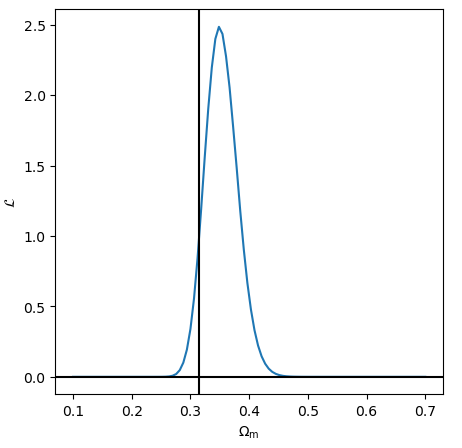
\includegraphics[width=\textwidth]{MainLayout/BORG_chapter/figures/omega_m_L.png}
        \caption{Likelihood profile for $\Omega_m$}
        \label{fig:omega_m_lpt_L}
    \end{subfigure}
    \hfill
    \begin{subfigure}{0.45\textwidth}
        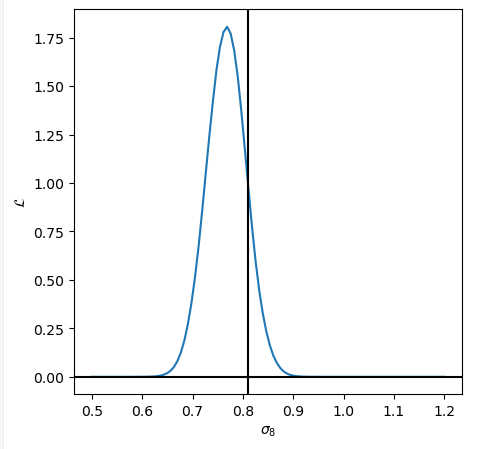
\includegraphics[width=\textwidth]{MainLayout/BORG_chapter/figures/sigma_8_L.png}
        \caption{Likelihood profile for $\sigma_8$}
        \label{fig:sigma8_lpt_L}
    \end{subfigure}
    \caption{Likelihood profiles of the cosmological parameters for a synthetic N-body simulation generated with LPT}
    \label{fig:cosmo_lpt_L}
\end{figure}

\begin{figure}
    \centering
    \begin{subfigure}{0.45\textwidth}
        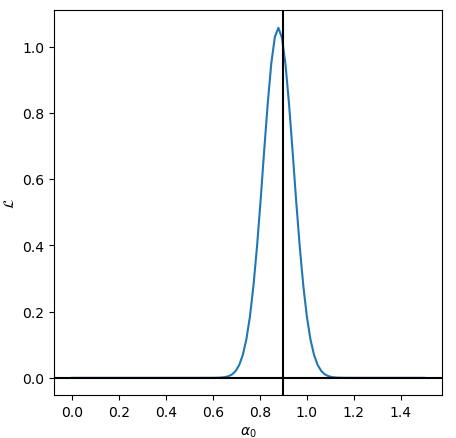
\includegraphics[width=\textwidth]{MainLayout/BORG_chapter/figures/alpha_L.png}
        \caption{Likelihood profile for $\alpha$}
        \label{fig:alpha_lpt_L}
    \end{subfigure}
    \hfill
    \begin{subfigure}{0.45\textwidth}
        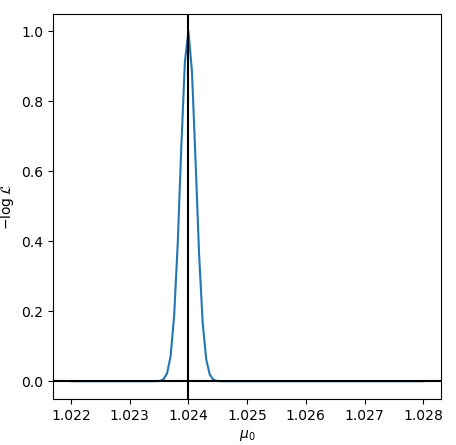
\includegraphics[width=\textwidth]{MainLayout/BORG_chapter/figures/muA_L.png}
        \caption{Likelihood profile for $\mu_A$}
        \label{fig:muA_lpt_L}
    \end{subfigure}
    \caption{Likelihood profiles of $\alpha$ and $\mu_A$ for a synthetic N-body simulation generated with LPT}
    \label{fig:params1_lpt_L}
\end{figure}

\begin{figure}
    \centering
    \begin{subfigure}{0.45\textwidth}
        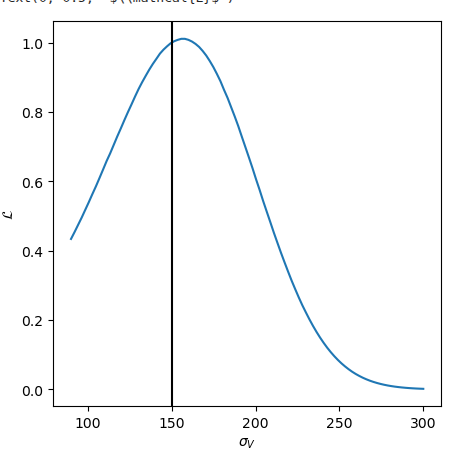
\includegraphics[width=\textwidth]{MainLayout/BORG_chapter/figures/sigma_v_L.png}
        \caption{Likelihood profile for $\sigma_v$}
        \label{fig:sigma_v_lpt_L}
    \end{subfigure}
    \hfill
    \begin{subfigure}{0.45\textwidth}
        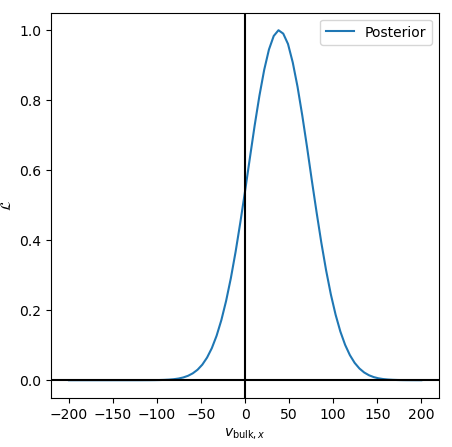
\includegraphics[width=\textwidth]{MainLayout/BORG_chapter/figures/bulk_x_L.png}
        \caption{Likelihood profile for $V_x$}
        \label{fig:Vx_lpt_L}
    \end{subfigure}
    \caption{Likelihood profiles $\sigma_v$ and $V_x$ for a synthetic N-body simulation generated with LPT}
    \label{fig:params2_lpt_L}
\end{figure}

\begin{figure}
    \centering
    \begin{subfigure}{0.45\textwidth}
        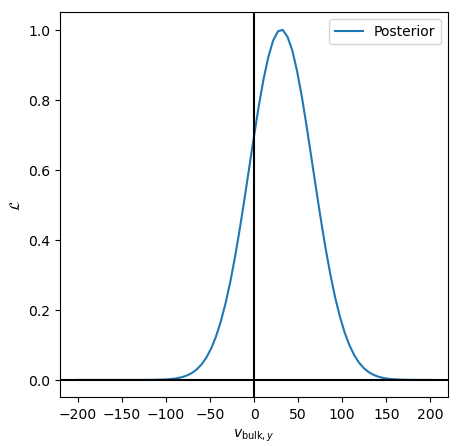
\includegraphics[width=\textwidth]{MainLayout/BORG_chapter/figures/bulk_y_L.png}
        \caption{Likelihood profile for $V_y$}
        \label{fig:Vy_lpt_L}
    \end{subfigure}
    \hfill
    \begin{subfigure}{0.45\textwidth}
        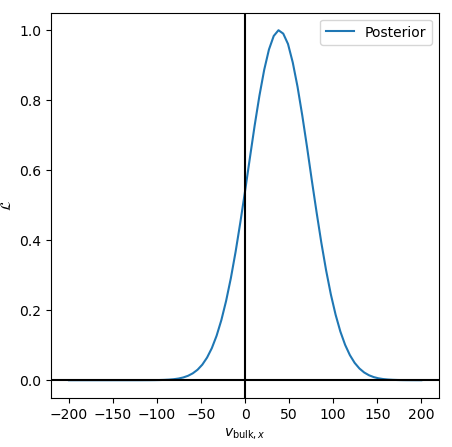
\includegraphics[width=\textwidth]{MainLayout/BORG_chapter/figures/bulk_x_L.png}
        \caption{Likelihood profile for $V_z$}
        \label{fig:Vz_lpt_L}
    \end{subfigure}
    \caption{Likelihood profiles $V_z$ and $V_z$ for a synthetic N-body simulation generated with LPT}
    \label{fig:params3_lpt_L}
\end{figure}

\section{Results of the field level inference on Uchuu-ZTF simulations}

We present in this section the results obtained on the DC PV. The procedure follows closely what was done on the self consistent simulations. 
The priors set on the parameters are:
\begin{itemize}
    \item $\alpha \sim \mathcal{U}[0.5, \, 2.5]$
    \item $\mu_A \sim \mathcal{U}[0.5, \, 1.5]$
    \item $\sigma_v \sim \mathcal{U}[50, \, 400] \, \text{km.s}^{-1}$
    \item Each bulk flow component $\sim \mathcal{U}[-200, \, +200] \, \text{km.s}^{-1}$ 
    \item $\Omega_m \sim \mathcal{U}[0.1, \, 0.8]$
    \item $\sigma_8 \sim \mathcal{U}[0.1, \, 1.5]$
\end{itemize}

The inference runs in four steps: 
\begin{enumerate}
 \item An initial warm-up phase is dedicated to sample the initial density perturbations $\delta^{IC}$ while all of other parameters are fixed using an LPT gravity solver. 
 This is done in 1000 MCMC steps.
 \item The following step we simultaneously $\delta^{IC}$ alongside nuisance and model parameters, specifically 
 $\sigma_v$, bulk flow, $\alpha$ and $\mu_A$ also using LPT. This is done for 3000 MCMC steps. 
 \item We keep on sampling the same parameters but switch to COLA for the gravity solver. The idea is that since LPT is much faster than COLA, to use it to initially guess some 
 of the model parameters so that sampling the parameters is then easier with COLA. For this run, it was done for 800 MCMC steps. 
 \item Lastly, we sample all of the parameters simultaneously including $\Omega_m$ and $\sigma_8$ using COLA. This step 
 takes a lot of computational on CPU. A converged state would be achieved during the timeline of this PhD. Efforts to parallelize the computations on GPUs is ongoing to accelerate this step.
\end{enumerate}
In Figure \ref{fig:dens_ztf_evolution} we display the evolution of the mean density field $\delta^{F}$ within a slice at the center of the box.


First, we present the results obtained when using the LPT gravity solver. 
We show in Figures \ref{fig:ztf_dens} slices of the final reconstructed density field with BORG in comparison with the Uchuu 
density. The red-dashed circle represents the limit of where the supernova are being generated (up to $z=0.06$). \\

\begin{figure}[htpb]
    \centering
    \begin{subfigure}{1\textwidth}
        \centering
        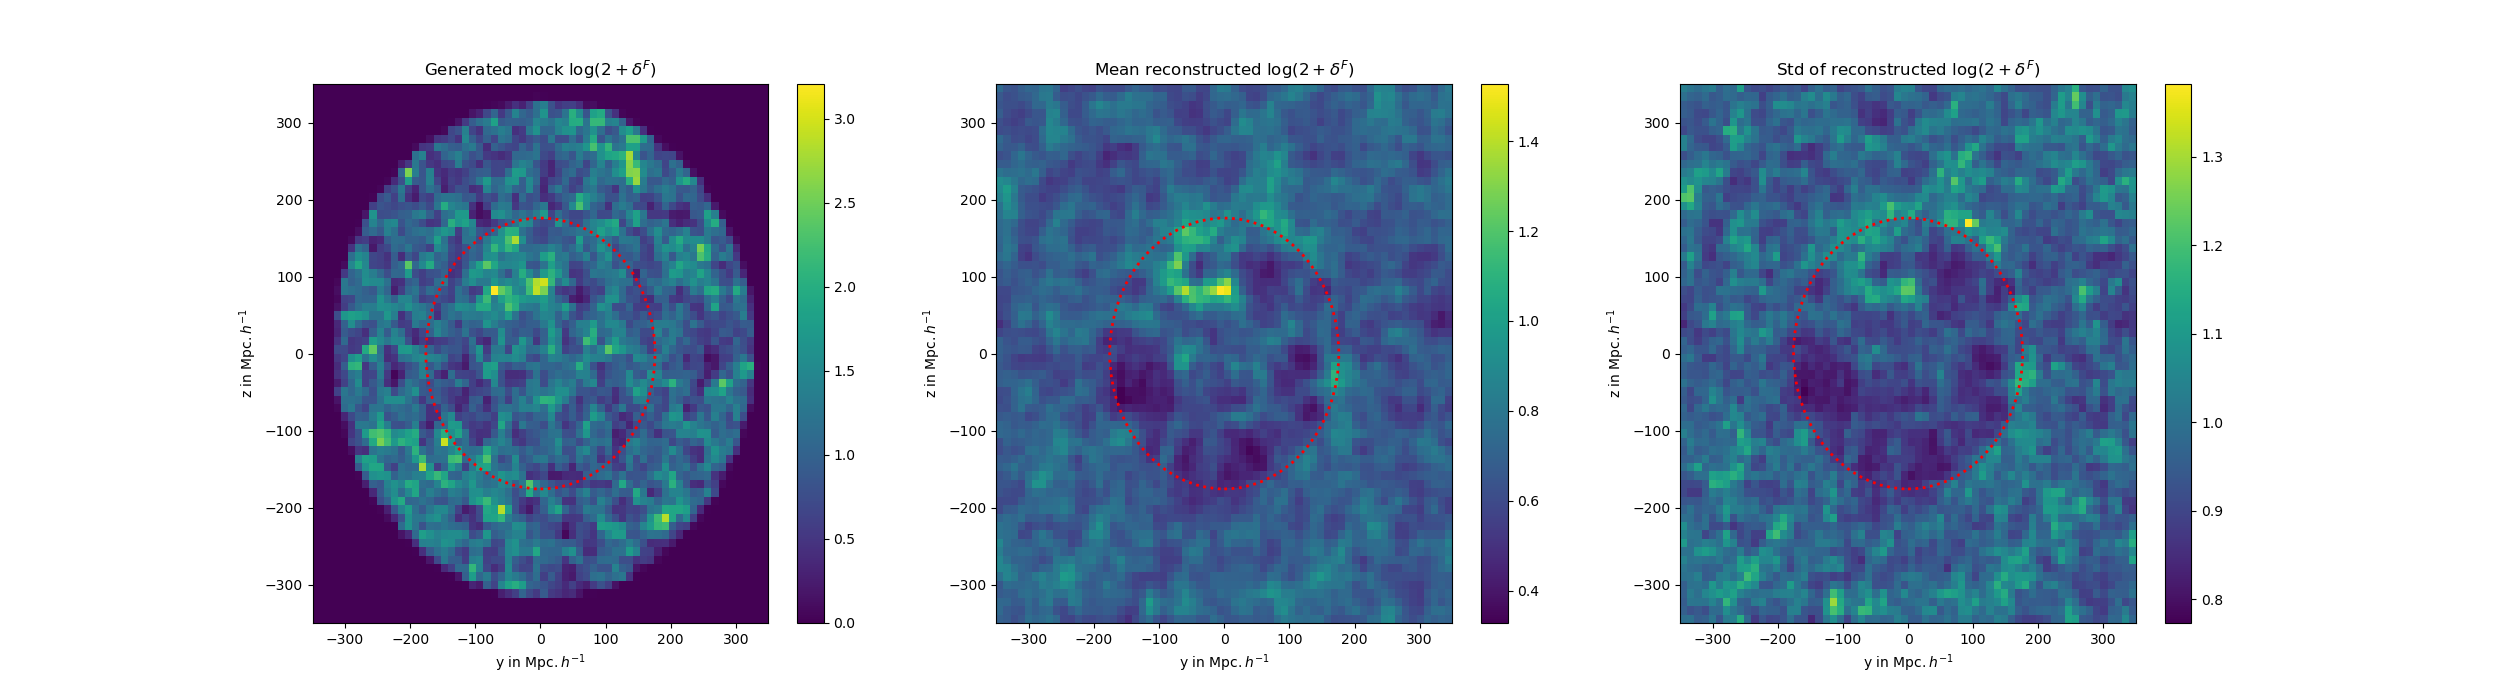
\includegraphics[width=1.2\textwidth]{MainLayout/BORG_chapter/figures/dens_slice_x_28.png}
        \caption{}
        \label{fig:ztf_dens_1}
    \end{subfigure}%
    
    \vspace{1em}
    
    \begin{subfigure}{1\textwidth}
        \centering
        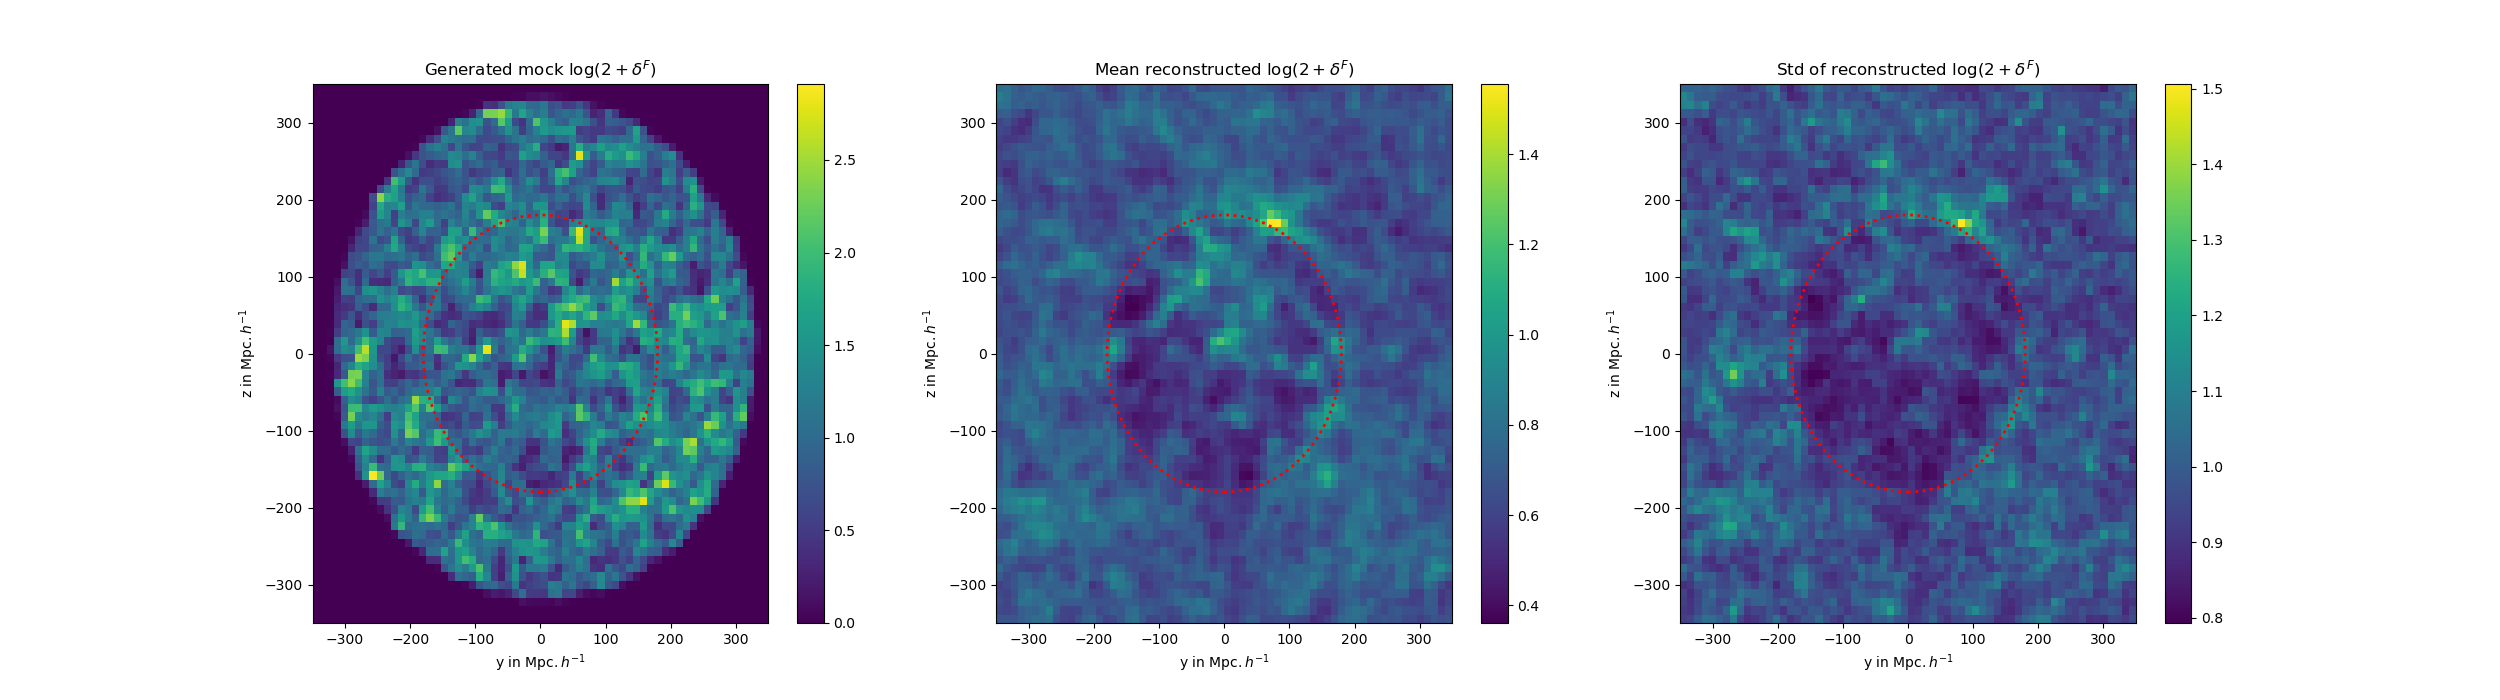
\includegraphics[width=1.2\textwidth]{MainLayout/BORG_chapter/figures/dens_slice_x_32.png}
        \caption{}
        \label{fig:ztf_dens_2}
    \end{subfigure}
    \caption{Slices of the density field from Uchuu and BORG reconstruction after having gone a CIC mass assignment. 
    The left column shows the Uchuu density field. The center column shows the mean posterior from BORG. 
    The right column shows the standard deviation. Each row is a different slice in the box.}
    \label{fig:ztf_dens}
    \end{figure}


We notice that the field reconstructed with BORG-PV manages to capture 
some of the underlying structure visible in Uchuu by comparing the overdense and underdense regions within the red-dashed circle. 
Notably, it is the largest structures that are 
recovered while smal scales structures seem to be missed. 
We show in Figures \ref{fig:ztf_vel} slices of the final reconstructed velocity field with BORG in comparison with the Uchuu 
velocity. \\ 

\begin{figure}[htpb]
    \centering
    \begin{subfigure}{1\textwidth}
        \centering
        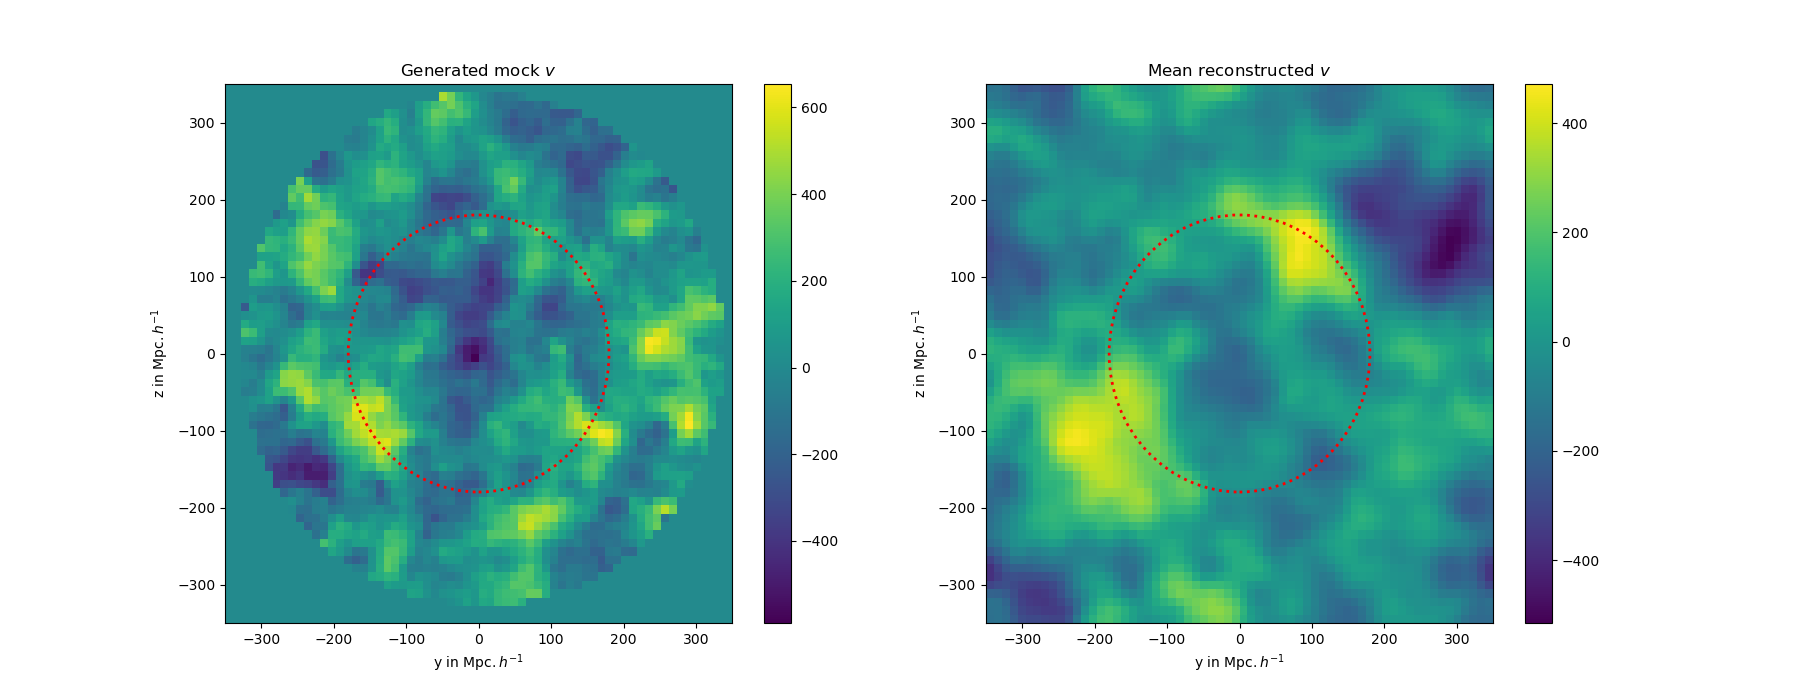
\includegraphics[width=1.0\textwidth]{MainLayout/BORG_chapter/figures/vel_slice_x_32.png}
        \caption{}
        \label{fig:ztf_vel_1}
    \end{subfigure}%
    
    \vspace{1em}
    
    \begin{subfigure}{1\textwidth}
        \centering
        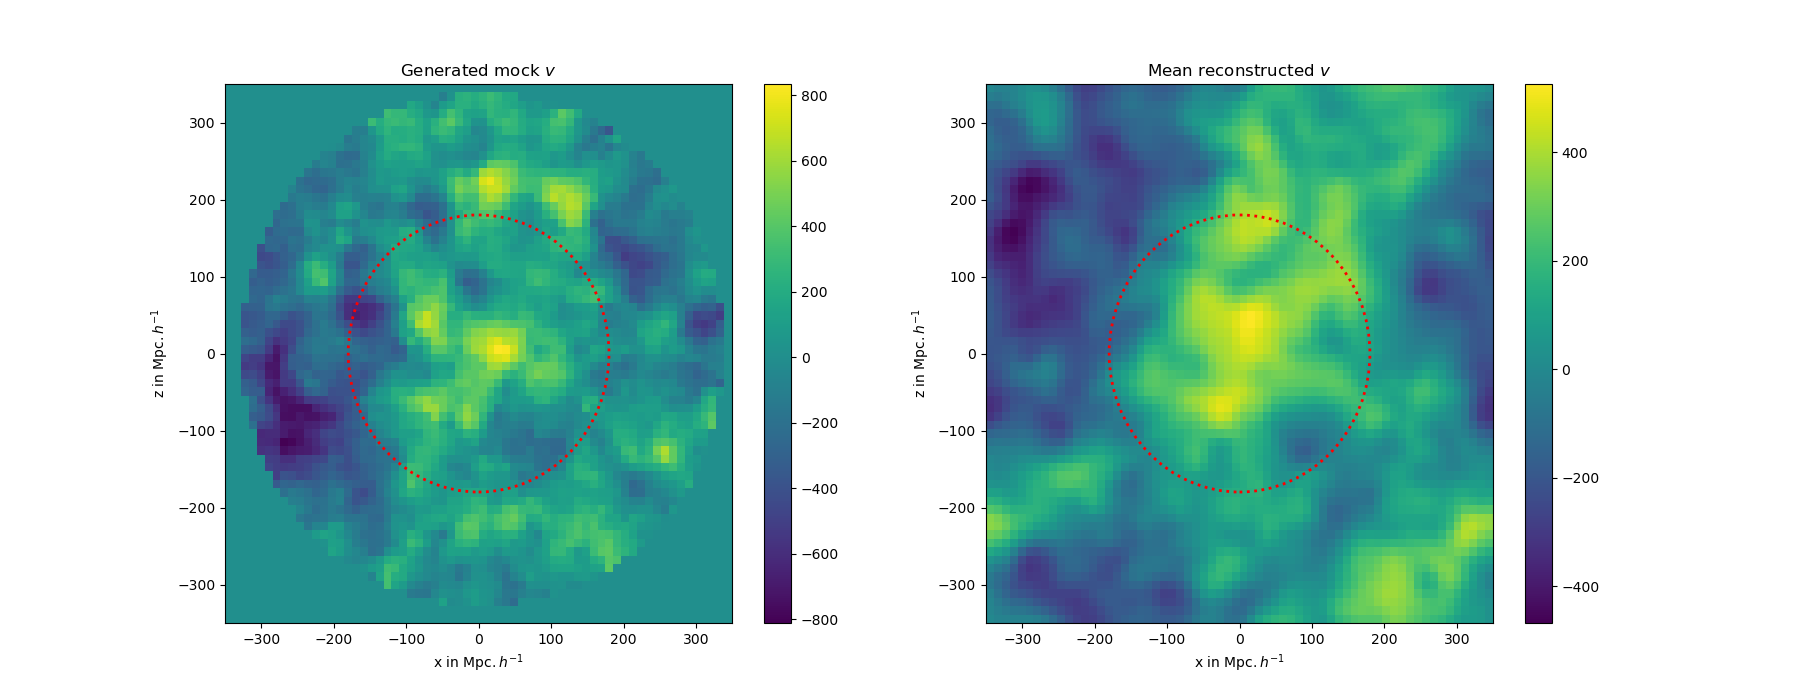
\includegraphics[width=1.0\textwidth]{MainLayout/BORG_chapter/figures/vel_slice_y_32.png}
        \caption{}
        \label{fig:ztf_vel_2}
    \end{subfigure}
    \caption{Slices of the velocity field from Uchuu and BORG reconstruction after having gone a CIC mass assignment. 
    The left column shows the Uchuu velocity field. The reight column shows the mean posterior from BORG. 
    Each row is a different slice in the box. The first row is a slice in the $x$ axis. The second row is a slice in the $y$ axis.}
    \label{fig:ztf_vel}
    \end{figure}



Similarly to the density field reconstruction, the BORG velocity field seems to match the Uchuu velocity at large scales. 
It is important to note that the velocity field 
is known to be more linear and Gaussian than the density field. 

---More results needed from here on out
To quantify this, we compare the power spectra of the density and velocity field components $v_x$, $v_y$ and $v_z$ from Uchuu to the one inferred by BORG in Figures (ref) as well 
as the cross correlation factor between them $r$ in Figures (ref). 
We notice that the power spectrum of the matter density matches the Uchuu power spectrum up to a wavenumber of $k \approx$. For the velocity fields we notice a matching result up 
to a wavenumber of $k \approx$. This confirms our qualitative results mentioned previously when looking directly at the reconstructed fields. \\

%Secondly we look at the sampled parameters. \\


%NEED SOME COLA RESULTS TO BETTER WRITE OFF THIS PART

%- results
% - covariance additions ?
% - full dataset with selection?

%\section{BONUS IF THERE IS TIME: Comparison with other methods for $f\sigma_8$}

%\textit{As with the self consistent simulation, we are restricted to a $\Lambda-CDM$ cosmology. Therefore if assume that $f\sigma_8$ is expressed as:}
%\begin{equation}
%    f \sigma_8 = \Omega_m^{0.55} \sigma_8
%\end{equation}
%\textit{by calculating this quantity, we can compare with other methods within the ZTF collaboration used to calculate $f\sigma_8$. Currently there is one ongoing work in doing so conducted by 
%Rafel Kebadian (Kebadian et al. in prep) where $f\sigma_8$ is determined using a maximum likelihood method on the DC PV supernovae. We present in Figure (ref) the results from the different methods. 
%We (hope) to see that using a field-level inference we obtain tighter constraints on $f\sigma_8$. However as mentioned before, we are limited to $\Lambda$CDM, so any deviations from 
%the expected value do not indicate what the strength of the underlying gravitational theory should be as much as it is a test on knowing whether the assumed gravitational theory (GR) 
%is correct or not. The maximum likelihood method however does not present that issue, but the $f\sigma_8$ constraints are looser.}